\documentclass[preview,border=5pt]{standalone}
\usepackage{teaching}
\begin{document}

\centering

\begin{tikzpicture}[scale=3, inner sep=0.1mm]
\draw[fill=blue!22.5!white] (0.25,0) arc (0:60:0.25cm) -- (0,0);
\draw [->,thick] (0,0) -- (0.5,{sqrt(3)/2});
\draw [->,thick] (0,0) -- (1,0);
\node at (1.1,0) {$\mathbf{a}$};
\node at (0,0.3) {$\mathbf{b}$};
\node at (0.8,0.3) {\small $\theta = \cos^{-1}\left(\dfrac{\mathbf{a}\cdot\mathbf{b}}{|\mathbf{a}||\mathbf{b}|}\right)$};

\end{tikzpicture}


\end{document}